\documentclass{beamer}
\hypersetup{pdfstartview={Fit}}

\usepackage[french]{babel}
\usepackage[T1]{fontenc}
\usepackage[utf8]{inputenc}

\usepackage{amsmath}
\usepackage{amssymb}
\usepackage{amsthm}


% quelques définitions
\theoremstyle{plain}
\newtheorem{thm}{Théorème}
\newtheorem{prop}{Proposition}

\theoremstyle{definition}
\newtheorem{defi}{Définition}
\newtheorem{qst}{Question}
\newtheorem{rmq}{Remarque}

\DeclareMathOperator\Var{Var}
\DeclareMathOperator\Cov{Cov}



\usetheme{Montpellier}
\usecolortheme{whale}


\title{Reconnaissance faciale par Eigenfaces}
\author{Bouarah Romain \and Langdorph Matthieu \and Ketels Lucas \and Nathan Souffan }
\date{\today}

\begin{document}


\begin{frame}[plain]
  \titlepage
\end{frame}


\section{Introduction}
% LUCAS
\subsection{Motivation}
\subsection{Histoire}

\section{Calcul des eigenfaces}
\subsection{Travail dans $\mathbb{R}^{N \times N}$}
\begin{frame}
  \frametitle{Représentation matricielle des images}
  \begin{defi}
    Une image de taille $N \times N$ est représentée par une matrice $N \times N$.\\
    Chaque coefficient représente un niveau de gris d'un pixel.
  \end{defi}
\end{frame}



\begin{frame}
  \frametitle{Transformation en un vecteur de $\mathbb{R}^{N \times N}$}
  On juxtapose simplement les colonnes de la matrice l'une en dessous de l'autre.
  \[
    \begin{pmatrix}
      p_{1,1} & p_{1,2} & \cdots & p_{1,N} \\
      p_{2,1} & p_{2,2} & \cdots & p_{2,N} \\
      \vdots  & \vdots  & \ddots & \vdots  \\
      p_{N,1} & p_{N,2} & \cdots & p_{N,N}
    \end{pmatrix}
    \rightarrow
    \begin{pmatrix}
      p_{1,1} \\
      p_{2,1} \\
      \vdots \\
      p_{N,1} \\
      \vdots \\
      p_{1,N} \\
      \vdots \\
      p_{N,N}
    \end{pmatrix}
  \]  
\end{frame}



\subsection{Matrice de covariance}



\begin{frame}  
  \frametitle{Observation sur les images des visages}
  \begin{qst}
    Que dire de la position de nos images de visages dans l'espace $\mathbb{R}^{N \times N}$?
  \end{qst}
  \pause
  \begin{exampleblock}{Réponse}
    Nos images de visages ne sont pas si éloignées les unes des autres. 
  \end{exampleblock}
\end{frame}



\begin{frame}
  \frametitle{Définition de la Matrice de Covariance}  
  \begin{defi}
    La matrice de covariance d'un vecteur de $p$ variables aléatoires $\overrightarrow{X} =
    \begin{pmatrix}
      X_1 \\
      \vdots \\
      X_p
    \end{pmatrix}$ dont chacune possède une variance, est la matrice carrée dont le terme générique est donné par $a_{i,j} = \Cov(X_i,X_j)$.
  \end{defi}
\end{frame}



\begin{frame}
  \frametitle{Encodons cette dispersion}  
  \begin{defi}[Estimation de la Matrice de Covariance]
    En partant d’un échantillon de réalisations indépendantes d’un vecteur aléatoire, une estimation de la matrice de covariance est donné par :
    \[
      \Var(\overrightarrow{X}) = \frac{1}{n} \displaystyle\sum_{i=1}^{n} (\overrightarrow{X_i} - \overrightarrow{\mu})(\overrightarrow{X_i}-\overrightarrow{\mu})^T
    \]
    où $\overrightarrow{\mu} = \frac{1}{n} \displaystyle\sum_{i=1}^{n}\overrightarrow{X_i}$ est le vecteur des moyennes empiriques.
  \end{defi}
\end{frame}



\begin{frame}
  \frametitle{Application à notre cas}
  Soit $I = [I_1,I_2,\dotsc,I_M]$ la matrice de l'ensemble de nos images.
  \begin{enumerate}
  \item<2-> On calcule le visage moyen $\Psi = \frac{1}{M}\displaystyle\sum_{i=1}^{M} I_i$.
  \item<3-> Chaque visage différe donc de la moyenne par le vecteur $\Phi_i = I_i - \Psi$.
  \item<4-> On calcule la matrice de covariance
    \[
      C = \frac{1}{M} \displaystyle\sum_{i=1}^{M} \Phi_i \Phi_i^T = \frac{1}{M} AA^T 
    \]
    où $A = [\Phi_1,\Phi_2,\dotsc,\Phi_M]$.    
  \end{enumerate}
\end{frame}



\begin{frame}
  \frametitle{Observations sur la Matrice de Covariance}
  La matrice de covariance $C$ est :
  \begin{itemize}
  \item<2-> symétrique réelle.
  \item<3-> définie semi-positive.
  \end{itemize}
\end{frame}



\subsection{Analyse en composantes principales}



\begin{frame}
  \frametitle{Introduction à l'Analyse en Composantes Principales}
  \begin{block}{Principe}
    Trouver des axes décrivant au mieux notre nuage de points.
  \end{block}
  \pause
  \begin{defi}[Eigenfaces]
    La méthode développéee par Turk et Pentland définit les \emph{eigenfaces} comme les axes principaux de l'ACP.
  \end{defi}
\end{frame}



\begin{frame}
  \frametitle{Illustration en 2 Dimensions}
  \begin{figure}
    \begin{overprint}
      \onslide<1>\centering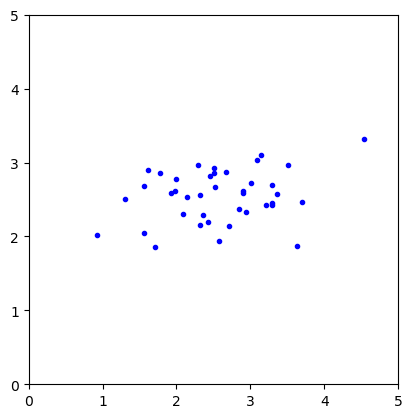
\includegraphics[scale=0.5]{src/beamer/figures/fig_pca_1.png}
      \onslide<2>\centering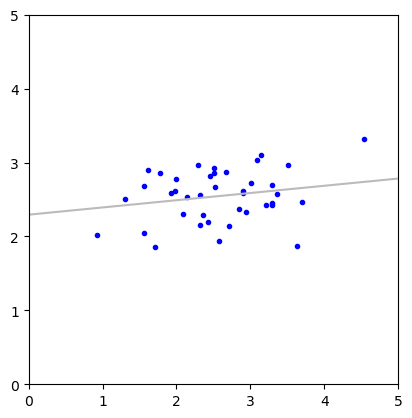
\includegraphics[scale=0.5]{src/beamer/figures/fig_pca_2.png}
      \onslide<3>\centering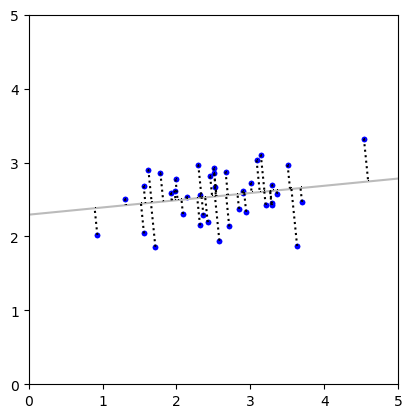
\includegraphics[scale=0.5]{src/beamer/figures/fig_pca_3.png}
    \end{overprint}
  \end{figure}
\end{frame}



\begin{frame}
  \begin{figure}
    \centering
    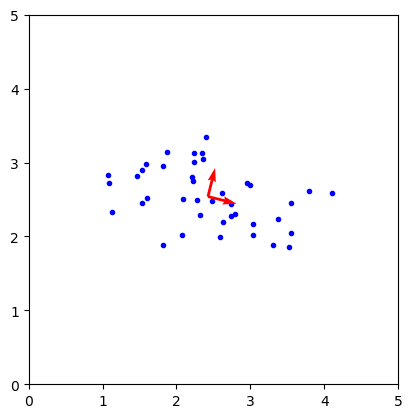
\includegraphics[scale=0.5]{src/beamer/figures/fig_pca_4.png}  
  \end{figure}
\end{frame}



\begin{frame}
  \frametitle{Limite de la Méthode}
  \begin{qst}
    Quels sont les problèmes de la méthode ?
  \end{qst}

  \pause
  
  \begin{exampleblock}{Réponse}
    \begin{itemize}
    \item La matrice de covariance est de taille $N^2 \times N^2$.
      \pause
    \item La diagonaliser est infaisable informatiquement.
    \end{itemize}
  \end{exampleblock}
\end{frame}



\subsection{Décomposition en valeurs singulières}
\begin{frame}
  \frametitle{\'{E}noncé de la Décomposition en Valeurs Singulières}
  \begin{thm}
    Soit $M$ une matrice $m \times n$, alors il existe une décomposition de la forme
    \[
      M = U \Sigma V^t
    \]
    avec $U$ et $V$ des matrices orthonormales de taille respectives $m \times m$ et $n \times n$.
  \end{thm}
  
  \begin{prop}
    \begin{itemize}
    \item les colonnes de $V$ sont les vecteurs propres de $M^TM$
    \item les colonnes de $U$ sont les vecteurs propres de $MM^T$
    \end{itemize}
  \end{prop}
\end{frame}


\section{Classification des visages}
% NATHAN
\subsection{Projection dans l'espace des visages}
\begin{frame}
  \frametitle{Projection d'un visage}
  Soit $\Gamma$ une nouvelle image de visage, on la projette dans l'espace des visages par :
  \[
    \omega_k = u_k^T(\Gamma - \Psi)
  \]
  \pause
  Pour $k \in \{1,\dotsc,M'\}$, on a alors :
  \[W =
    \begin{pmatrix}
      \omega_1 \\
      \vdots \\
      \omega_{M'}
    \end{pmatrix}
  \]
\end{frame}
\subsection{Analyse de la projection}


\begin{frame}
  \frametitle{Conclusion}
  \resizebox{\linewidth}{!}{
    \begin{tabular}{ | l | c | c | }
      \hline
                                      & proche d'une classe de visage & éloigné d'une classe de visage \\
      \hline
      proche de l'espace des visages  & \onslide<2->{visage connu}    & \onslide<3->{visage inconnu}   \\
      \hline
      éloigné de l'espace des visages & \onslide<4->{faux positif}    & \onslide<5->{pas un visage}    \\
      \hline
    \end{tabular}
  }
\end{frame}

\section{Application}
\subsection{Techniques utilisées aujourd'hui}
\subsection{Par les téléphones}

\section{Conclusion}
\subsection{Risque de la reconnaissance faciale}
\subsection{Références}

\begin{frame}
\end{frame}

\end{document}